\section{Appendix}

\begin{frame}{Limitations (\danger) and Future Work (\VarClock)}

  \begin{columns}[c,onlytextwidth]
\begin{column}{0.49\textwidth}
\begin{itemize}
    \item[\danger] Iceberg pruning may remove low-support (potential exact overlap) concepts
    \begin{itemize}
      \item \textcolor{rosa}{Lowest} non-trivial \textcolor{rosa}{expert concepts} contain $1000$ documents 
      \item \textit{Most} \textcolor{blau}{lowest data-driven concepts} contain less than $1000$ documents
      \item[$\rightarrow$] Jaccard similarity $\overset{!}{<} 1$
      \item[$\rightarrow$] No difference for consistency lattice
    \end{itemize}
    \item[\VarClock] Compare more than two knowledge sources
    \item[\VarClock] Explore alternative overlap measures beyond Jaccard similarity
\end{itemize}
\end{column}
\begin{column}{0.49\textwidth}
  \vspace{-1em}
  \begin{figure}
\centering
\includegraphics[width=\textwidth,height=0.4\textheight,keepaspectratio]{resources/banksearch/ground_truth/mlb_expanded_colored_lowest_layer.pdf}
\caption{Complete expert lattice {\tiny[\hyperlink{appendix:expert-lattice-detail}{Details}]}.}
\end{figure}
\vspace{-3em}
\begin{figure}
\centering
\includegraphics[width=\textwidth,height=0.38\textheight,keepaspectratio]{resources/banksearch/topic_model/banksearch_0.05_iceberg_colored_lowest_layer.pdf}
\caption{Data-driven iceberg lattice \tiny[\hyperlink{appendix:topic-model-details}{Details}].}
\end{figure}
\end{column}
\end{columns}

\end{frame}

\begin{frame}[fragile]{Case Study: BankSearch Dataset Example File {\tiny[\hyperlink{main:dataset-overview}{Back to dataset overview}]}}

\begin{lstlisting}[language=BankSearchHTML,basicstyle=\ttfamily\tiny]
ID=H0302
URL=http://www.klab.caltech.edu/~koch/biophysics-book/biophysics-book-review-marder.html
SIZE=12894
DATE=11/07/2002
TIME=17:03:40
DATASET=Biology
HTML=<HTML><HEAD>
<TITLE>In search of computation</TITLE>
</HEAD>
<BODY BGCOLOR="#FFFFFF" background="/images/back_cream.gif">
...
<A HREF="http://neurosci.nature.com/">
<IMG SRC="/images/bar_home_u.gif" WIDTH="108" HEIGHT="34" BORDER="0" ALT="nature neuroscience"></A>
...
<P><I>The Biophysics of Computation</I> includes full and mathematically rigorous treatments of many topics that are found conventionally in neuroscience texts, such as passive cable theory, synaptic physiology, mechanisms of synaptic plasticity, gating of ion channels and mechanisms of action potential initiation and propagation.
...
This respect will ensure that the book will have credibility with its biological audience. Equally importantly, the respect and appreciation that Koch shows for the biological literature teaches young theorists that the aim is to understand the deep mysteries of how the brain computes, not deny them.</P>
...
<FONT SIZE=2 face=Verdana,geneva,arial,sans-serif>Copyright 1999 Nature America Inc.</FONT></TD>
</TR>
</TABLE>

</BODY>
</HTML>
\end{lstlisting}

\end{frame}


\begin{frame}{Case Study: BankSearch Dataset Details}
\hypertarget{appendix:dataset-detail}{}
\begin{itemize}
    \item 11\,000 documents
    \item 14 categories
    \begin{itemize}
      \item \textcolor{blue}{Three} categories are not assigned to documents\\
       {
      \small
      \begin{tabular}{ll}
          \toprule
          \textbf{Top-Category} & \textbf{Sub-Category} \\
          \midrule
          \textcolor{blue}{Finance} & Commercial Banks, Building Societies, Insurance Agencies\\
          \textcolor{blue}{Science} & Astronomy, Biology \\
          \textcolor{blue}{Programming} & C/C++, Java, Visual Basic \\
          Sport & Soccer, Motor Racing \\
          \bottomrule
      \end{tabular}
      }
    \end{itemize}
   
    \item 1000 documents per category
    \item Expert hierarchy is mapped to document-level \ac{mlb} constraints
    \item Mapping yields 81 \ac{mlb} constraints
\end{itemize}

\vfill
{\tiny[\hyperlink{main:dataset-overview}{Back to dataset overview}]}
\end{frame}

\begin{frame}{Case Study: BankSearch Dataset Details}
\hypertarget{appendix:dataset-detail2}{}

\begin{table}
\centering
\caption{Expert-defined vs.\ data-driven topic assignments $\mathcal{T}$ for BankSearch ($n=11\,000$ documents), where $s_{\min}$ denotes the support of the smallest topic.}
\label{tab:compare-expert-data-driven}

\resizebox{\columnwidth}{!}{%
\begin{tabular}{lrrrrrr}
\toprule
Type
& $|\mathcal{T}|$
& $\overline{n}_{\mathrm{docs/topic}}$
& $n_{\min}$
& $s_{\min}$
& $n_{\max}$
& $\overline{n}_{\mathrm{topics/doc}}$ \\
\midrule
Expert
& 11 & 1000.0 & 1000 & 0.091 & 1000 & 1.00 \\
Data-driven topic model
& 11 & 2202.9 & 412 & 0.037 & 3555 & 2.20 \\
\bottomrule
\end{tabular}%
}
\end{table}

\vfill
{\tiny[\hyperlink{main:dataset-overview}{Back to dataset overview}]}
\end{frame}





\begin{frame}{MLB Constraints $\Sigma$: Formal Properties}
\hypertarget{appendix:mlb-defs}{}

\begin{columns}[T,onlytextwidth]
\begin{column}{0.53\textwidth}
\begin{itemize}
    \item Let $\Sigma \subseteq G \times G \times G$ be a set of \ac{mlb} constraints, cluster hierarchy $H$
    \item $MLB_{x y z}=(d_x,d_y,d_z)$ means $d_x$ and $d_y$ are closer to each other than to $d_z$
    \item BankSearch dataset: 81 \ac{mlb} constraints
\end{itemize}
\end{column}
\begin{column}{0.45\textwidth}
\banksearchHierarchyToMLB{}
\end{column}
\end{columns}

\begin{block}{\ac{mlb} Implication}
Given \ac{mlb} constraint $MLB_{x y z}$:
$\forall c \in H:\ d_x \in c \wedge d_z \in c \rightarrow d_y \in c$
\end{block}

\begin{block}{\ac{mlb} Counterexample}
Given \ac{mlb} constraint $MLB_{x y z}$:
$\exists c \in H:\ d_x \in c \wedge d_y \in c \wedge d_z \notin c$
\end{block}

\vfill
{\tiny[\hyperlink{main:mlb-constraints}{Back to MLB overview}]}
\end{frame}

\begin{frame}{Closure Operator $\phi_{\Sigma}$: Proof}
\hypertarget{appendix:closure-proof}{}
\begin{itemize}
    \item A set $A \subseteq G$ is $\Sigma$-consistent iff every constraint in $\Sigma$ is respected:
    \[
      \forall(d_x,d_y,d_z)\in\Sigma:\ \{d_x,d_z\}\subseteq A \Rightarrow d_y\in A .
    \]
    \item Let $\mathcal{S}_{\Sigma}$ be the family of all $\Sigma$-consistent subsets of $G$.
    \begin{itemize}
      \item[$\Rightarrow$] $G \in \mathcal{S}_{\Sigma}$
      \item[$\Rightarrow$] For any $\Sigma$-consistent sets $\{C_i\}_{i\in I}$ (i.e., $C_i \in \mathcal{S}_{\Sigma} \forall i \in I$):\\
      Their intersection $D = \bigcap_{i \in I} C_i$ and
      some constraint $(d_x, d_y, d_z) \in \Sigma$ with $\{d_x, d_z\} \subseteq D$: 
      \begin{itemize}
      \item[$\overset{\mathrm{Def.}}{\Rightarrow}$] $\{d_x, d_z\} \subseteq C_i \forall i \in I$
      \item[$\Rightarrow$] $C_i \in \mathcal{S}_{\Sigma} 
      \Rightarrow d_y \in C_i \forall i \in I 
      \Rightarrow d_y \in D 
      \Rightarrow D$ is $\Sigma$-consistent (i.e., $D \in \mathcal{S}_{\Sigma}$)
      \end{itemize}
    \end{itemize}
    \item $\mathcal{S}_{\Sigma}$ is closed under intersection $\Rightarrow \mathcal{S}_{\Sigma}$ is a closure system
    \item Associated closure operator $\phi_{\Sigma}(A)=\bigcap \{ S \in \mathcal{S}_{\Sigma} \mid A \subseteq S \}$
    \begin{itemize}
      \item $\phi_{\Sigma}$ is extensive, monotone, and idempotent $\qed$
    \end{itemize}

\end{itemize}
\vfill
{\tiny[\hyperlink{main:mlb-constraints}{Back to MLB overview}]}
\end{frame}

\begin{frame}{Structural Saturation}
\hypertarget{appendix:saturation}{}
\begin{itemize}
    \item Standard \ac{fca} closure operators work on flat implications (i.e., $d_x \wedge d_z \rightarrow d_y$)
    \item Hierarchical constraints imply transitive implications 
    \item[\danger] Transitive implications not naturally listed
    \item[$\rightarrow$] Structural saturation: Explicitly add implicitly implied transitive inference rules
    \item Closure operator $\phi_{\Sigma}$ is applied to updated saturated implication set
\end{itemize}

\vspace{0.35em}
\begin{center}
\begin{tikzpicture}[
    node distance=1.25cm,
    box/.style={draw,rounded corners=2pt,align=center,minimum width=2.7cm,minimum height=0.75cm},
    arr/.style={-{Latex[length=2mm]},thick}
]
\node[box] (i1) {$a,b \Rightarrow c$};
\node[box,below=0.45cm of i1] (i2) {$b,c \Rightarrow d$};
\node[box,right=1.8cm of $(i1)!0.5!(i2)$] (i3) {$a,b \Rightarrow d$};
\coordinate (i3upper) at ($(i3.west)!0.25!(i3.north west)$);
\coordinate (i3lower) at ($(i3.west)!0.25!(i3.south west)$);
\draw[arr] (i1.east) -- (i3upper);
\draw[arr] (i2.east) -- (i3lower);
\end{tikzpicture}
\end{center}
\vfill
{\tiny[\hyperlink{main:mlb-constraints}{Back to MLB overview}]}
\end{frame}

\begin{frame}{Expert Lattice: Details}
  \hypertarget{appendix:expert-lattice-detail}{}
\begin{columns}[c,onlytextwidth]
\begin{column}{0.49\textwidth}
\begin{itemize}
  \item 15 attributes
  \item Correspondence to ground-truth topics via matching extents (i.e., documents)
  \begin{itemize}
    \item $M3$: \texttt{Biology}
    \item $M4$: \texttt{Astronomy}
    \item $M0 \cap M2$: \texttt{Motor Racing}
    \item $M1 \cap M2$: \texttt{Soccer}
    \item $M0 \cap M1$: \texttt{Sport}
    \item $M5 \cap M7$: \texttt{C/C++}
    \item $M6 \cap M7$: \texttt{Java}
    \item $M5 \cap M6$: \texttt{Visual Basic}
    \item $M10 \cap M11$: \texttt{Commercial Banks}
    \item $M9 \cap M10$: \texttt{Insurance Agencies}
    \item $M9 \cap M11$: \texttt{Building Societies}
  \end{itemize}
  % \item 
\end{itemize}
\end{column}
\begin{column}{0.49\textwidth}
\begin{figure}
\centering
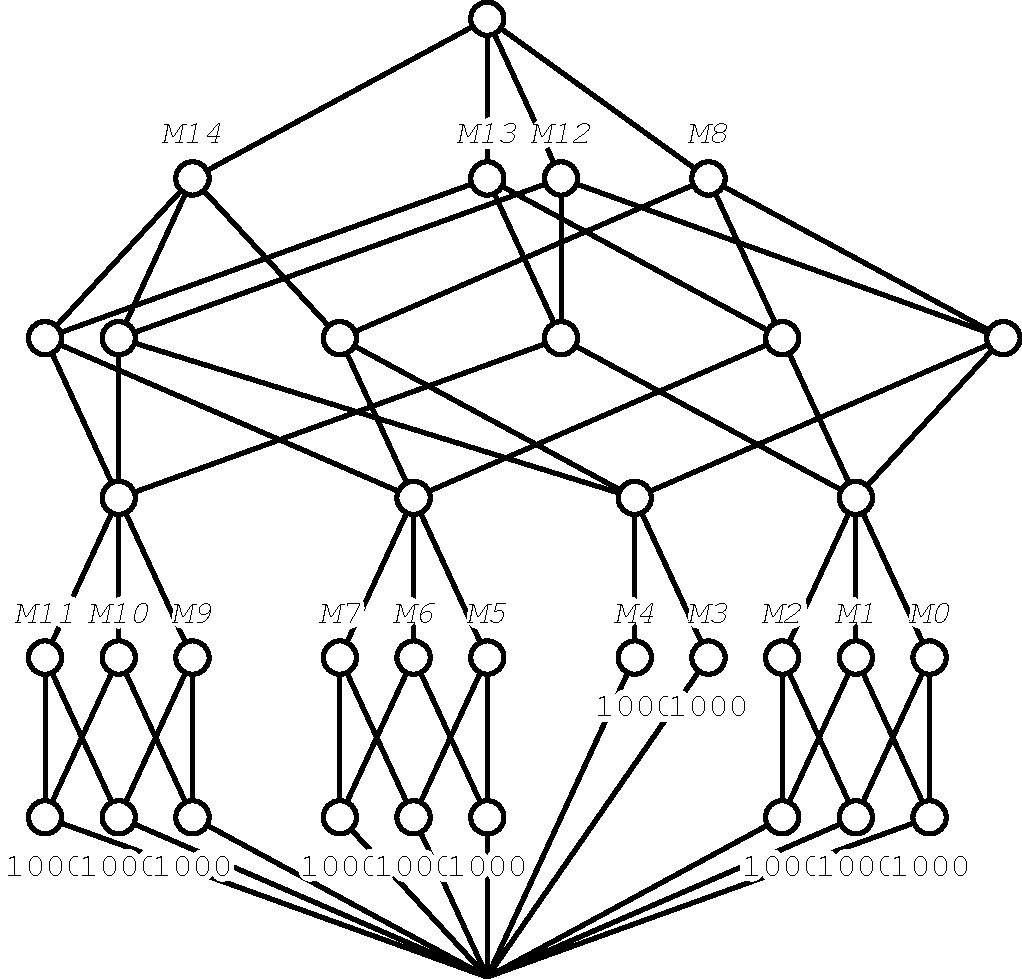
\includegraphics[width=\textwidth,height=0.58\textheight,keepaspectratio]{resources/banksearch/ground_truth/mlb_expanded.pdf}
\caption{Expert lattice.}
\end{figure}
\end{column}
\end{columns}

\vspace{0.55em}
{\small 
Top labels denote attributes, bottom labels indicate the number of documents in the concept extent.
}
\vfill
{\tiny[\hyperlink{main:comp-lattices}{Back to overview}]}
\end{frame}


\begin{frame}{Data-Driven Topic Lattice: Details}
  \hypertarget{appendix:topic-model-details}{}
  \begin{columns}[T,onlytextwidth]
\begin{column}{0.70\textwidth}
\begin{itemize}
    \item {\small \texttt{Gensim}}'s \ac{lda} represents documents as a mixture of $T$ latent topics 
    \begin{itemize}
      \item $T=11 = \#$ BankSearch categories
    \end{itemize}
    \item Binary formal context $\Theta \in \mathbb{R}^{D \times T}$ by thresholding document-topic probabilities at $\delta_t=0.07$
    \begin{itemize}
      \item Elbow criterion
      \item Density above $0.2$
      \item If no topic exceeds $\delta_t=0.07$, set highest probability topic $1$
    \end{itemize}
    \item Iceberg concept lattice (via TITANIC~\cite{stumme_titanic_2002}): keep concepts $(A,B)$ with support $\text{supp}(B)=\frac{|B'|}{|G|} \ge \delta_{ms}=0.05$ 
    \begin{itemize}
      \item Elbow criterion
      \item $24$ concepts
      \item Concepts do not correspond to original category clusters
    \end{itemize}
\end{itemize}
\vfill
{\tiny[\hyperlink{main:topic-model-overview}{Back to overview}]}
\end{column}
\begin{column}{0.3\textwidth}
  \vspace{-1.4em}
\begin{center}
\includegraphics[height=0.43\textheight]{incidence_density_vs_threshold_svg-tex.pdf}
\hfill
\includegraphics[height=0.43\textheight]{concepts_vs_support_svg-tex.pdf}
\end{center}
\end{column}
\end{columns}
\end{frame}



\begin{frame}{Consistency Lattice $\mathcal{C}_{\cap}$}
\hypertarget{appendix:consistency-detail}{}

    Let $\mathcal{C}_{\Sigma}$ be the expert \ac{mlb} closure system and $\mathcal{C}_{TM}$ the topic-model closure system $TM$. 

\[
\mathcal{C}_{\cap}
= \mathcal{C}_{\Sigma}\cap\mathcal{C}_{TM}
= \{A\subseteq G \mid \phi_{\Sigma}(A)=A \land \phi_{TM}(A)=A\}
\]

\begin{itemize}
  \item Closure operator $\phi_{\cap}$ is the limit of alternating composition of $\phi_{\Sigma}$ and $\phi_{TM}$
  \begin{itemize}
    \item Let $X_{k+1} =\phi_{TM}(\phi_{\cap}(X_k))$, where $X_0 = X \subseteq G$
  \item Fixpoint $\phi_\cap(X) = \lim_{k\to\infty} (\phi_{TM} \circ \phi_\Sigma)^k(X)$
  \end{itemize}
  \item[$\rightarrow$] generated concepts are valid under both $\Sigma$ and data-driven topic-model $TM$
  \vspace{1em}
  \item[\danger] Computationally expensive
  \item[$\rightarrow$] Instead of generating all closed sets and filtering them post-hoc, employ optimized version of Ganters Next-Closure algorithm
  \begin{itemize}
    \item Only use $\cap$-irreducible extents $A \in C_{\cap}$ (i.e., cannot be represented as intersection of strict supersets: $I_{sup}(A) \supsetneq A$):
    \[
    I_{sup}(A) = \bigcap_{g \in G \setminus A} \phi_\cap(A \cup \{g\})
    \]
  \end{itemize}
\end{itemize}
\vfill
{\tiny[\hyperlink{main:consistency-overview}{Back to consistency lattice overview}]}
\end{frame}


\begin{frame}{BankSearch Agreement Matrix}
  \hypertarget{appendix:agreement-heatmap}{}
\begin{columns}[T,onlytextwidth]
\begin{column}{0.43\textwidth}
\begin{itemize}
  \item Jaccard similarity between all concept extents
    \item Most non-trivial expert \& data-driven concept pairs have near-zero overlap
    \item Only five non-trivial pairs exceed $J(A,B)>0.5$
    \item[$\rightarrow$] Coherence lattice instead of consistency lattice
\end{itemize}
\vfill
{\tiny Back to \dots}\\
{\tiny [\hyperlink{main:coherence-lattice}{coherence lattice foundations}]}\\
{\tiny [\hyperlink{main:coherence-findings}{coherence lattice findings}]}
\end{column}
\begin{column}{0.55\textwidth}
\centering
\includegraphics[width=\textwidth,height=0.68\textheight,keepaspectratio]{heatmap_0.05_svg-tex.pdf}
\end{column}
\end{columns}
\end{frame}
